\section{累计偏差与鞅收敛}
\label{sec:dtsp-deviation}

鞅把一个累计过程中“无法预测的部分”单独分离出来。接下来要问它会偏离起点多远。这里有两类不同的问题。第一类固定一段有限的运行，问整段运行中的最大偏差超过某个阈值的概率有多大；它给出有限预算下的概率保证。第二类让运行时间趋于无穷，问累计量是否有极限、极限的期望是否等于原来的期望；它给出渐近结论。前者不能由后者推出，后者也不能由前者推出，本节分别建立。

\subsection{最大偏差与尾概率}
\label{sec:dtsp-maximal-tail}
\label{sec:rv-anytime}
\label{sec:stoch-self-normalized-adaptive-design}

\paragraph{从终点误差到全程最大误差}
设一个在线程序每一步都更新累计误差$M_n$，用户随时可能查看。只控制终点$M_n$并不够：路径可能在中途偏得很远又折回来。最直接的办法是对每个时刻分别用Chebyshev不等式再求并，但这样得到的界会随查看次数$n$线性变大。鞅结构允许做得好得多。图~\ref{fig:dtsp-doob-maximal}(a)给出想法：在路径首次越过阈值的时刻$\tau$停下来，事件“前$n$步的最大值越过阈值”恰好是$\{\tau\leq n\}$，而停下时的值至少是阈值。于是控制最大值的问题变成了控制一个停止过程，而停止过程的期望由可选抽样掌握。

\begin{theorem}[Doob最大不等式]
  \label{thm:dtsp-doob-maximal}
  设$(X_n)$是次鞅，$x>0$。则
  \[
    x\,\mathbb P\Bigl(\max_{k\leq n}X_k\geq x\Bigr)\leq\mathbb E\Bigl[X_n;\max_{k\leq n}X_k\geq x\Bigr]\leq\mathbb EX_n^{+}.
  \]
  特别地，若$(M_n)$是平方可积鞅，则
  \begin{equation}
    \mathbb P\Bigl(\max_{k\leq n}|M_k|\geq x\Bigr)\leq\frac{\mathbb EM_n^2}{x^2},\qquad
    \mathbb E\Bigl[\max_{k\leq n}M_k^2\Bigr]\leq4\,\mathbb EM_n^2.
    \label{eq:dtsp-doob-l2}
  \end{equation}
\end{theorem}

\begin{proof}
令$\tau=\inf\{k:X_k\geq x\}$，$A=\{\max_{k\leq n}X_k\geq x\}=\{\tau\leq n\}$。$\tau\wedge n\leq n$是有界停时，$A\in\mathcal F_{\tau\wedge n}$。由定理~\ref{thm:dtsp-bounded-optional-sampling}的次鞅形式，$\mathbb E[X_n\mid\mathcal F_{\tau\wedge n}]\geq X_{\tau\wedge n}$，于是
\[
  \mathbb E[X_n\mathbb I_A]\geq\mathbb E[X_{\tau\wedge n}\mathbb I_A]=\mathbb E[X_\tau\mathbb I_A]\geq x\,\mathbb P(A),
\]
最后一步因为在$A$上$X_\tau\geq x$。第二个不等号由$X_n\mathbb I_A\leq X_n^{+}$得到。

对平方可积鞅，$M_n^2$是次鞅，把第一部分用于$M_n^2$与阈值$x^2$即得第一式。对第二式记$M^\ast=\max_{k\leq n}|M_k|$，它满足$\mathbb E(M^\ast)^2\leq\sum_{k\leq n}\mathbb EM_k^2<\infty$。次鞅$|M_k|$的第一部分给出$x\,\mathbb P(M^\ast\geq x)\leq\mathbb E[|M_n|;M^\ast\geq x]$。乘以$2$并对$x>0$积分，用Fubini定理交换次序：
\[
  \begin{aligned}
    \mathbb E(M^\ast)^2&=\int_0^\infty2x\,\mathbb P(M^\ast\geq x)\,\mathrm dx
    \leq2\,\mathbb E\Bigl[|M_n|\int_0^{M^\ast}\mathrm dx\Bigr]\\
    &=2\,\mathbb E[|M_n|M^\ast]
    \leq2\sqrt{\mathbb EM_n^2}\sqrt{\mathbb E(M^\ast)^2}.
  \end{aligned}
\]
最后一步是Cauchy--Schwarz不等式。两边除以有限的$\sqrt{\mathbb E(M^\ast)^2}$（为零时结论平凡）再平方，得到常数$4$。
\end{proof}

式~\eqref{eq:dtsp-doob-l2}的第一式与只对终点用Chebyshev不等式得到的界完全相同：对鞅而言，控制整段路径的最大值不需要付出额外代价。图~\ref{fig:dtsp-doob-maximal}(b)用$n=100$步的公平游走核对：阈值$x=20$时，整段最大偏差超过阈值的模拟频率约为$0.092$，终点超过阈值约为$0.059$，Doob界给出$100/400=0.25$。界是保守的，但它对所有平方可积鞅都成立，只用到了终点的二阶矩。

\begin{figure}[htbp]
  \centering
  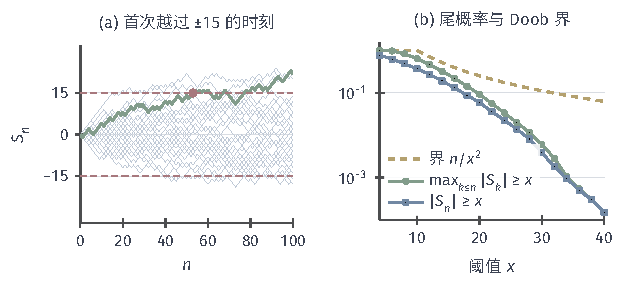
\includegraphics[width=106mm]{figures/03-optimization-evolution-and-signals/02-processes-and-trajectory-evolution/tikz/dtsp-doob-maximal/figure.pdf}
  \caption{Doob最大不等式。$S_n$为公平$\pm1$游走，$n=100$。(a)$40$条模拟路径，绿色路径在红点处首次达到$|S_k|\geq15$，在那里停止即把最大值事件化为停止事件；(b)$20000$次模拟得到的$\mathbb P(\max_{k\leq n}|S_k|\geq x)$与$\mathbb P(|S_n|\geq x)$，黄色虚线为界$\min\{1,n/x^2\}$。}
  \label{fig:dtsp-doob-maximal}
\end{figure}

\paragraph{非负超鞅的越界：Ville不等式}
同一想法用于非负超鞅，还能把有限时段推广到全部时刻。这一形式将成为指数型界的统一出口。

\begin{theorem}[Ville不等式]
  \label{thm:dtsp-ville}
  设$(L_n)_{n\geq0}$是非负超鞅，$x>0$。则
  \[
    \mathbb P\Bigl(\sup_{n\geq0}L_n\geq x\Bigr)\leq\frac{\mathbb EL_0}{x}.
  \]
\end{theorem}

\begin{proof}
固定$0<x'<x$，令$\tau=\inf\{n:L_n\geq x'\}$。由超鞅的有界可选抽样，$\mathbb EL_{\tau\wedge n}\leq\mathbb EL_0$；由非负性，$L_{\tau\wedge n}\geq x'\,\mathbb I\{\tau\leq n\}$。所以$x'\,\mathbb P(\tau\leq n)\leq\mathbb EL_0$，令$n\to\infty$得$\mathbb P(\tau<\infty)\leq\mathbb EL_0/x'$。事件$\{\sup_nL_n\geq x\}$包含于$\{\tau<\infty\}$，因为上确界达到$x$意味着某个时刻超过$x'$。再令$x'\uparrow x$即得结论。引入$x'$是为了处理上确界只被逼近、不在任何时刻取到的情形。
\end{proof}

这条不等式在后文统称为\term{Ville不等式}（Ville's inequality）。若取$\mathbb EL_0\leq1$和$x=1/\delta$，它说非负超鞅在整个无穷时段中曾经达到$1/\delta$的概率至多$\delta$。下面的指数型界都按同一模式构造：先找一个以累计误差为指数的非负超鞅，再用Ville不等式读出概率。

\paragraph{有界增量：Azuma--Hoeffding不等式}
第一个指数界只假设每步增量落在已知长度的区间里。它需要一个关于单个变量的引理：均值为零、取值区间长度不超过$c$的变量，其指数矩不超过同方差尺度的高斯变量。

\begin{lemma}[条件Hoeffding引理]
  \label{lem:dtsp-conditional-hoeffding}
  设$\mathcal G$是子$\sigma$代数，$D$可积且$\mathbb E[D\mid\mathcal G]=0$。若存在对$\mathcal G$可测的$a\leq b$使$a\leq D\leq b$几乎必然，且$b-a\leq c$，$c$为常数，则对所有$\gamma\in\mathbb R$，
  \[
    \mathbb E[e^{\gamma D}\mid\mathcal G]\leq\exp\Bigl(\frac{\gamma^2c^2}{8}\Bigr)\qquad\text{几乎必然}.
  \]
\end{lemma}

\begin{proof}
在$\{a=b\}$上，$D=a$且条件均值为零，故$D=0$，结论平凡。以下在$\{a<b\}$上论证。指数函数是凸的，对$a\leq x\leq b$它位于连接两端点的弦下方：
\[
  e^{\gamma x}\leq\frac{b-x}{b-a}e^{\gamma a}+\frac{x-a}{b-a}e^{\gamma b}.
\]
代入$x=D$并对$\mathcal G$取条件期望；$a,b$对$\mathcal G$可测可以提出，$\mathbb E[D\mid\mathcal G]=0$，得到$\mathbb E[e^{\gamma D}\mid\mathcal G]\leq(be^{\gamma a}-ae^{\gamma b})/(b-a)$。记$\theta=-a/(b-a)\in[0,1]$、$s=\gamma(b-a)$，右侧的对数为$\psi(s)=\log\bigl[(1-\theta)e^{-\theta s}+\theta e^{(1-\theta)s}\bigr]$。直接求导可得$\psi(0)=\psi'(0)=0$，且$\psi''(s)=r(1-r)\leq1/4$，其中$r=\theta e^s/(1-\theta+\theta e^s)\in[0,1]$。由Taylor公式的积分余项，$\psi(s)\leq s^2/8\leq\gamma^2c^2/8$。
\end{proof}

\begin{theorem}[Azuma--Hoeffding不等式]
  \label{thm:dtsp-azuma}
  设$(M_n)$是鞅，$M_0=0$，鞅差满足$a_k\leq D_k\leq b_k$，其中$a_k,b_k$对$\mathcal F_{k-1}$可测且$b_k-a_k\leq c_k$，$c_k$为常数。记$C_n=\sum_{k\leq n}c_k^2>0$。则对$x>0$，
  \begin{equation}
    \mathbb P\Bigl(\max_{k\leq n}M_k\geq x\Bigr)\leq\exp\Bigl(-\frac{2x^2}{C_n}\Bigr).
    \label{eq:dtsp-azuma}
  \end{equation}
\end{theorem}

\begin{proof}
固定$\gamma>0$，令$L_k=\exp\bigl(\gamma M_k-\gamma^2\sum_{j\leq k}c_j^2/8\bigr)$。由引理~\ref{lem:dtsp-conditional-hoeffding}，$\mathbb E[L_k\mid\mathcal F_{k-1}]=L_{k-1}\mathbb E[e^{\gamma D_k}\mid\mathcal F_{k-1}]e^{-\gamma^2c_k^2/8}\leq L_{k-1}$，所以$(L_k)$是非负超鞅，$L_0=1$。对$k\leq n$有$\sum_{j\leq k}c_j^2\leq C_n$，因此在事件$\{\max_{k\leq n}M_k\geq x\}$上$\max_{k\leq n}L_k\geq\exp(\gamma x-\gamma^2C_n/8)$。Ville不等式给出
\[
  \mathbb P\Bigl(\max_{k\leq n}M_k\geq x\Bigr)\leq\exp\Bigl(-\gamma x+\frac{\gamma^2C_n}{8}\Bigr),
\]
取$\gamma=4x/C_n$即得式~\eqref{eq:dtsp-azuma}。
\end{proof}

证明没有用到鞅差之间的独立性，只用到“给定过去后均值为零、范围受控”。对独立有界变量，它退化为Hoeffding不等式。代价是它按每一步可能的最坏范围计费：只要增量可能取到$\pm1$，就按方差$1$的尺度算，哪怕这件事极少发生。

\paragraph{条件方差：Freedman不等式}
考虑一个稀疏下注的例子：每一步以$0.95$的概率不下注，以各$0.025$的概率赢或输$1$，共$n=1000$步。增量范围是$[-1,1]$，Azuma界为$\exp(-x^2/2000)$；但每步条件方差只有$0.05$，实际的累计方差只有$50$，远小于范围给出的$1000$。图~\ref{fig:dtsp-azuma-freedman}显示$x=30$时精确尾概率约为$1.8\times10^{-5}$，Azuma界却是$0.64$，几乎没有信息。要利用小的条件方差，需要把第~\ref{sec:dtsp-quadratic-variation}节的可预测二次变差放进指数超鞅。

\begin{figure}[htbp]
  \centering
  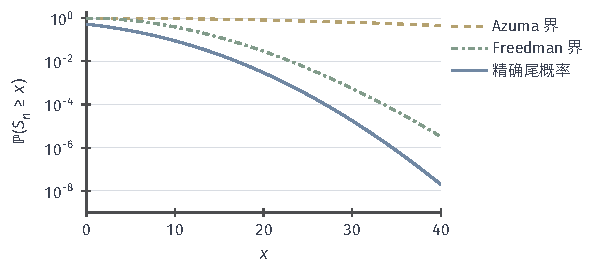
\includegraphics[width=100mm]{figures/03-optimization-evolution-and-signals/02-processes-and-trajectory-evolution/tikz/dtsp-azuma-freedman/figure.pdf}
  \caption{稀疏下注的尾概率与两种界（精确计算）。每步增量以概率$0.025$取$+1$、以$0.025$取$-1$、以$0.95$取$0$，$n=1000$。蓝线为由卷积精确算出的$\mathbb P(S_n\geq x)$；黄色虚线为Azuma界$\exp(-x^2/2n)$；绿色点划线为Freedman界$\exp\{-x^2/[2(v+x/3)]\}$，$v=50$为累计条件方差。纵轴为对数刻度。}
  \label{fig:dtsp-azuma-freedman}
\end{figure}

\begin{theorem}[Freedman不等式]
  \label{thm:dtsp-freedman}
  设$(D_k)$是鞅差，$|D_k|\leq b$几乎必然，$b>0$。记$S_n=\sum_{k\leq n}D_k$，$V_n=\langle S\rangle_n=\sum_{k\leq n}\mathbb E[D_k^2\mid\mathcal F_{k-1}]$。则对任意$x,v>0$，
  \begin{equation}
    \mathbb P\bigl(\exists n\geq1:\ S_n\geq x,\ V_n\leq v\bigr)\leq\exp\Bigl(-\frac{x^2}{2(v+bx/3)}\Bigr).
    \label{eq:dtsp-freedman}
  \end{equation}
\end{theorem}

\begin{proof}
先证一个标量不等式：对$0<\gamma<3/b$和$|u|\leq b$，
\[
  e^{\gamma u}\leq1+\gamma u+\frac{\gamma^2u^2}{2(1-\gamma b/3)}.
\]
展开指数级数，$k\geq2$项满足$(\gamma u)^k/k!\leq\frac{(\gamma u)^2}{2}(\gamma b/3)^{k-2}$，因为$k!\geq2\cdot3^{k-2}$；对$k\geq2$求和是一个几何级数。代入$u=D_k$并取条件期望，一次项消失，再用$1+t\leq e^t$：
\[
  \mathbb E[e^{\gamma D_k}\mid\mathcal F_{k-1}]\leq\exp\bigl(\phi(\gamma)\,\mathbb E[D_k^2\mid\mathcal F_{k-1}]\bigr),\qquad
  \phi(\gamma)=\frac{\gamma^2}{2(1-\gamma b/3)}.
\]
因此$L_n=\exp(\gamma S_n-\phi(\gamma)V_n)$是非负超鞅，$L_0=1$。在$\{S_n\geq x,V_n\leq v\}$上$L_n\geq\exp(\gamma x-\phi(\gamma)v)$，于是由Ville不等式，左侧概率不超过$\exp(-\gamma x+\phi(\gamma)v)$。取$\gamma=x/(v+bx/3)$，它落在$(0,3/b)$内，且$1-\gamma b/3=v/(v+bx/3)$，代入后指数恰为$-x^2/[2(v+bx/3)]$。
\end{proof}

Freedman界的分母有两项。小偏差时$v$主导，界像方差为$v$的高斯尾；大偏差时$bx/3$主导，界退化为指数尾，反映单步增量最多为$b$。对独立有界变量，$V_n$是确定数，式~\eqref{eq:dtsp-freedman}在固定$n$处给出Bernstein型不等式；对鞅，$V_n$随路径变化，事件中“$V_n\leq v$”这一项把界限定在实际波动不大的路径上。回到第~\ref{sec:dtsp-quadratic-variation}节领先时加注的赌徒：长期落后的路径$V_n$接近$n/4$，界随之收紧。

\paragraph{查看时刻与同时成立的保证}
上面三个界的时间量词不同，使用时要和查看方式对应。只在预先固定的时刻$n$查看，固定时刻的界就够了。若最多查看$T$次，可以给第$t$次分配失败概率$\delta_t$，只要$\sum_t\delta_t\leq\delta$，并合界就保证总失败概率不超过$\delta$。若查看时刻由数据决定，例如“第一次看起来足够好时停止”，就需要对所有时刻同时成立的保证：若$\mathbb P(\bigcup_{n\geq1}E_n)\leq\delta$，则对任何几乎必然有限的停时$\tau$都有$\mathbb P(E_\tau)\leq\delta$。Doob与Azuma界的最大值形式、Ville不等式和Freedman界都属于这一类，它们来自非负超鞅，而不是把固定时刻界中的$n$换成随机时刻。

\paragraph{可预测设计下的自归一化界}
在许多序贯问题中，每一步先根据历史选一个查询方向，再观测带噪响应。设参数$\bm\theta^\star\in\mathbb R^d$未知，第$k$步选择特征$\bm x_k\in\mathbb R^d$，观测
\begin{equation}
  y_k=\bm x_k^{\top}\bm\theta^\star+\varepsilon_k.
  \label{eq:stoch-adaptive-linear-observation}
\end{equation}
特征可以依赖此前的全部结果，但必须在$\varepsilon_k$揭晓之前确定，即$(\bm x_k)$可预测；噪声$\varepsilon_k$对$\mathcal F_k$可测。下面关心的累计量是噪声沿所选方向的加权和$\bm S_n=\sum_{k\leq n}\bm x_k\varepsilon_k$，它是历史适应的随机累计量。

先给噪声一个条件尾部假设。若存在$\sigma>0$，使对每个$k$和每个$\gamma\in\mathbb R$，
\begin{equation}
  \mathbb E[e^{\gamma\varepsilon_k}\mid\mathcal F_{k-1}]\leq\exp\Bigl(\frac{\gamma^2\sigma^2}{2}\Bigr)\qquad\text{几乎必然},
  \label{eq:dtsp-conditional-subgaussian}
\end{equation}
称$(\varepsilon_k)$为参数$\sigma^2$的\term{条件次高斯鞅差}（conditionally sub-Gaussian martingale difference）。名称中的“鞅差”是这一条件的推论：由$e^{\gamma u}\geq1+\gamma u$得$\gamma\,\mathbb E[\varepsilon_k\mid\mathcal F_{k-1}]\leq e^{\gamma^2\sigma^2/2}-1$，分别令$\gamma\downarrow0$与$\gamma\uparrow0$，得到条件均值为零。有界噪声由引理~\ref{lem:dtsp-conditional-hoeffding}满足此条件，高斯噪声取其方差即可。

特征可预测时，$\bm S_n$的每个坐标都是定理~\ref{thm:dtsp-martingale-transform}意义下的鞅变换。自然的误差尺度不是欧氏范数：某个方向被反复查询后，累计噪声在该方向上的规模也随之增长，应当按“该方向积累了多少信息”来归一化。取事先固定的$\lambda>0$，令
\[
  \bm V_n=\lambda\bm I+\sum_{k=1}^n\bm x_k\bm x_k^{\top},\qquad
  \lVert\bm S_n\rVert_{\bm V_n^{-1}}=\sqrt{\bm S_n^{\top}\bm V_n^{-1}\bm S_n}.
\]
$\bm V_n$在常被查询的方向上大，逆矩阵就在这些方向上小。用随机设计矩阵本身来度量累计噪声的做法称为\term{自归一化}（self-normalized）。

\begin{theorem}[向量自归一化界]
  \label{thm:dtsp-self-normalized}
  设$(\bm x_k)$可预测，$(\varepsilon_k)$满足式~\eqref{eq:dtsp-conditional-subgaussian}。则对任意$\delta\in(0,1)$，以至少$1-\delta$的概率，对所有$n\geq0$同时有
  \begin{equation}
    \lVert\bm S_n\rVert_{\bm V_n^{-1}}^2\leq2\sigma^2\log\Bigl(\frac{\det(\bm V_n)^{1/2}\det(\lambda\bm I)^{-1/2}}{\delta}\Bigr).
    \label{eq:stoch-vector-self-normalized-bound}
  \end{equation}
\end{theorem}

\begin{proof}
第一步，固定方向。对固定的$\bm u\in\mathbb R^d$，$\gamma_k=\bm u^{\top}\bm x_k$对$\mathcal F_{k-1}$可测。式~\eqref{eq:dtsp-conditional-subgaussian}对确定的$\gamma$成立；对只取有限个有理值的$\mathcal F_{k-1}$可测$\gamma_k$，在各取值事件上分别使用它即可；一般的$\gamma_k$用这类简单函数逐点逼近，再对每个$A\in\mathcal F_{k-1}$用Fatou引理，得到
\[
  \mathbb E\bigl[e^{\gamma_k\varepsilon_k-\sigma^2\gamma_k^2/2}\bigm|\mathcal F_{k-1}\bigr]\leq1.
\]
逐步相乘可知$L_n(\bm u)=\exp\bigl(\bm u^{\top}\bm S_n-\frac{\sigma^2}{2}\bm u^{\top}(\bm V_n-\lambda\bm I)\bm u\bigr)$是非负超鞅，$L_0(\bm u)=1$。

第二步，对所有方向取平均。固定方向只能控制一个投影；为同时控制所有方向，取与数据独立的高斯权重$\bm U\sim\mathcal N(\bm 0,(\sigma^2\lambda)^{-1}\bm I)$，定义$\overline L_n=\mathbb E_{\bm U}[L_n(\bm U)]$。非负性允许交换条件期望与对$\bm U$的积分（Tonelli定理），所以$\overline L_n$仍是非负超鞅，$\overline L_0=1$。把高斯密度与指数中的二次型合并，指数变为$\bm u^{\top}\bm S_n-\frac{\sigma^2}{2}\bm u^{\top}\bm V_n\bm u$，配方后积分得到
\[
  \overline L_n=\Bigl(\frac{\det(\lambda\bm I)}{\det(\bm V_n)}\Bigr)^{1/2}\exp\Bigl(\frac{\lVert\bm S_n\rVert_{\bm V_n^{-1}}^2}{2\sigma^2}\Bigr).
\]
行列式比来自两个高斯积分的归一化常数，指数项来自配方后中心的移动。

第三步，读出概率。由Ville不等式，$\mathbb P(\sup_n\overline L_n\geq1/\delta)\leq\delta$。在补事件上对所有$n$都有$\overline L_n<1/\delta$，取对数整理即为式~\eqref{eq:stoch-vector-self-normalized-bound}。
\end{proof}

各项假设各有分工。条件次高斯性构造每一步的指数超鞅；特征可预测性让$\bm x_k$在条件期望中被当作已知；$\lambda>0$使高斯混合与逆矩阵从$n=0$起就有定义。行列式$\det\bm V_n$记录各方向信息的共同增长：重复查询同一方向与首次查询新方向提供的信息不同，所以不能把它简单换成查询次数。这里只建立历史适应累计量的偏差界；据此为$\bm\theta^\star$构造置信集合、分析序贯决策的统计性质，属于统计推断与决策部分的任务。还应注意，这里的“自归一化”与第~\ref{sec:dtsp-importance}节自归一化重要性抽样中的“权重之和作分母”不是同一个对象。

\subsection{鞅的极限与期望保持}
\label{sec:dtsp-martingale-limits}

\paragraph{上穿次数}
现在让时间趋于无穷。一条实值路径没有极限，当且仅当它的下极限严格小于上极限；这时可以找到两个有理数$a<b$夹在中间，路径无穷多次从$a$以下走到$b$以上。把一次“从$\leq a$出发、到达$\geq b$”称为对区间$[a,b]$的一次\term{上穿}（upcrossing），记前$n$步完成的上穿次数为$U_n[a,b]$。图~\ref{fig:dtsp-upcrossings}(a)中，公平游走在$300$步内对$[-2,4]$完成了$3$次上穿。要证明收敛，只需证明对每一对有理数$a<b$，总上穿次数几乎必然有限。

上穿次数可以用一个下注策略来数：价格跌到$a$以下就买入，涨到$b$以上就卖出。每完成一次上穿至少赚$b-a$，最后一笔若尚未卖出，亏损不超过$(X_n-a)^-$。而这个策略只依据过去的价格决定是否持有，是可预测的；在超鞅（不利的市场）中，任何可预测的非负有界策略期望收益都不为正。两者对照，就得到上穿次数期望的界。

\begin{theorem}[Doob上穿不等式]
  \label{thm:dtsp-upcrossing}
  设$(X_n)$是超鞅，$a<b$。则$(b-a)\,\mathbb EU_n[a,b]\leq\mathbb E(X_n-a)^-$。
\end{theorem}

\begin{proof}
令$H_0=0$，并对$k\geq1$定义持有指示$H_k=\mathbb I\{H_{k-1}=1,X_{k-1}<b\}+\mathbb I\{H_{k-1}=0,X_{k-1}\leq a\}$：未持有时一旦价格$\leq a$就买入，持有时直到价格$\geq b$才卖出。$H_k$只用到$X_0,\ldots,X_{k-1}$，可预测，且取值于$\{0,1\}$。把收益$(H\cdot X)_n$按持有区间分组：每个完整的持有区间对应一次上穿，收益至少$b-a$；最后一个未结束的区间从某个$\leq a$的价格买入，收益至少$X_n-a\geq-(X_n-a)^-$。因此$(H\cdot X)_n\geq(b-a)U_n[a,b]-(X_n-a)^-$。由定理~\ref{thm:dtsp-martingale-transform}，$H\cdot X$是超鞅，$\mathbb E(H\cdot X)_n\leq0$，整理即得。
\end{proof}

\paragraph{几乎必然收敛}
上穿不等式把“无穷振荡”与“期望有界”对立起来。

\begin{theorem}[超鞅收敛定理]
  \label{thm:dtsp-supermartingale-convergence}
  设$(X_n)$是超鞅，且$\sup_n\mathbb EX_n^-<\infty$。则$X_n$几乎必然收敛到一个可积随机变量$X_\infty$。特别地，非负超鞅几乎必然收敛；满足$\sup_n\mathbb E|M_n|<\infty$的鞅几乎必然收敛。
\end{theorem}

\begin{proof}
对有理数$a<b$，$\mathbb E(X_n-a)^-\leq|a|+\mathbb EX_n^-$有与$n$无关的上界。由单调收敛，$\mathbb EU_\infty[a,b]=\lim_n\mathbb EU_n[a,b]<\infty$，所以$U_\infty[a,b]<\infty$几乎必然。可数多对有理数的例外集合之并仍是零概率事件，在其补集上$\liminf X_n=\limsup X_n$，即$X_n$在$[-\infty,\infty]$中有极限$X_\infty$。又$\mathbb E|X_n|=\mathbb EX_n+2\mathbb EX_n^-\leq\mathbb EX_0+2\sup_k\mathbb EX_k^-$，由Fatou引理$\mathbb E|X_\infty|\leq\liminf_n\mathbb E|X_n|<\infty$，所以极限几乎必然有限且可积。非负超鞅满足$X_n^-=0$；对鞅，把定理用于$M_n$本身即可。
\end{proof}

图~\ref{fig:dtsp-upcrossings}(b)是一个有界鞅的例子。坛子里起初有红、蓝球各一个，每次随机摸一个球，放回并再加入一个同色球。记摸了$n$次后红球比例为$F_n=R_n/(n+2)$，则$\mathbb E[F_{n+1}\mid\mathcal F_n]=(R_n+F_n)/(n+3)=F_n$，所以$(F_n)$是取值于$[0,1]$的鞅，必然几乎处处收敛。图中十二次实验的比例很快稳定下来，但稳定在不同的位置：极限是随机的，实际上服从$[0,1]$上的均匀分布。鞅收敛定理保证每条路径都会停下来，却不规定停在哪里。

\begin{figure}[htbp]
  \centering
  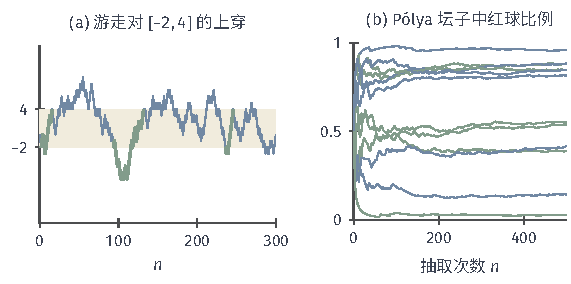
\includegraphics[width=97mm]{figures/03-optimization-evolution-and-signals/02-processes-and-trajectory-evolution/tikz/dtsp-upcrossings/figure.pdf}
  \caption{上穿与鞅收敛。(a)公平$\pm1$游走的一条$300$步模拟路径，绿色粗线标出对区间$[-2,4]$（黄色带）完成的上穿；游走不收敛，上穿次数随时间无限增长。(b)Pólya坛子（初始红、蓝各一球，每次加入一个与摸出球同色的球）中红球比例的$12$次模拟，比例是有界鞅，各自收敛到不同的随机极限。}
  \label{fig:dtsp-upcrossings}
\end{figure}

路径收敛并不意味着期望收敛。在“加倍或清零”的乘积鞅$M_n=\prod_{k\leq n}Y_k$中（$Y_k$等概率取$0,2$），只要出现一次$0$，此后就恒为零，所以$M_n\to0$几乎必然；但$\mathbb EM_n=1$对所有$n$成立。概率越来越小的路径上保留着越来越大的值，这部分期望在极限中消失了，与加倍下注中“跑到无穷远”的负质量是同一现象。

\paragraph{一致可积与平均收敛}
要让极限保持期望，就要排除上面这种期望集中在越来越小事件上的情形，这正是一致可积的含义。

\begin{theorem}[一致可积鞅]
  \label{thm:dtsp-ui-martingale}
  对鞅$(M_n)$，以下三条等价：(1)$(M_n)$一致可积；(2)$M_n$几乎必然且在$L^1$中收敛到某个$M_\infty$；(3)存在可积随机变量$Z$使$M_n=\mathbb E[Z\mid\mathcal F_n]$对所有$n$成立。此时$M_n=\mathbb E[M_\infty\mid\mathcal F_n]$，且$M_\infty=\mathbb E[Z\mid\mathcal F_\infty]$，其中$\mathcal F_\infty=\sigma(\bigcup_n\mathcal F_n)$。
\end{theorem}

\begin{proof}
(1)$\Rightarrow$(2)：一致可积推出$\sup_n\mathbb E|M_n|<\infty$，由定理~\ref{thm:dtsp-supermartingale-convergence}几乎必然收敛；几乎必然收敛加一致可积推出$L^1$收敛。(2)$\Rightarrow$(3)：对$A\in\mathcal F_n$与$m\geq n$，$\mathbb E[M_m\mathbb I_A]=\mathbb E[M_n\mathbb I_A]$；令$m\to\infty$，$L^1$收敛允许取极限，得$\mathbb E[M_\infty\mathbb I_A]=\mathbb E[M_n\mathbb I_A]$，所以$M_n=\mathbb E[M_\infty\mid\mathcal F_n]$，取$Z=M_\infty$。(3)$\Rightarrow$(1)：由条件Jensen不等式$|M_n|\leq\mathbb E[|Z|\mid\mathcal F_n]$，而$\{|M_n|>K\}\in\mathcal F_n$，故
\[
  \mathbb E[|M_n|;|M_n|>K]\leq\mathbb E[|Z|;|M_n|>K],\qquad\mathbb P(|M_n|>K)\leq\frac{\mathbb E|Z|}{K}.
\]
单个可积变量$|Z|$在小概率事件上的积分一致地小：对任意$\varepsilon>0$存在$\eta>0$，使$\mathbb P(A)<\eta$时$\mathbb E[|Z|;A]<\varepsilon$。取$K>\mathbb E|Z|/\eta$，便对所有$n$有$\mathbb E[|M_n|;|M_n|>K]<\varepsilon$。最后一句：$M_\infty$对$\mathcal F_\infty$可测，且对$A\in\bigcup_n\mathcal F_n$有$\mathbb E[M_\infty\mathbb I_A]=\mathbb E[Z\mathbb I_A]$；满足此等式的$A$构成$\lambda$系，而$\bigcup_n\mathcal F_n$是$\pi$系，由$\pi$-$\lambda$定理推广到$\mathcal F_\infty$。
\end{proof}

条件(3)说，一致可积鞅恰好是“对同一个终极量的逐步预测”。Pólya坛子比例有界，因而一致可积，$\mathbb EF_\infty=\mathbb EF_0=1/2$；乘积鞅$\prod Y_k$不一致可积，不能写成某个固定变量的条件期望。这也解释了定理~\ref{thm:dtsp-optional-stopping}的第三个条件：停止过程一致可积时，它是对$M_\tau$的逐步预测，期望得以保持。

\paragraph{平方可积鞅}
若有二阶矩的统一上界，结论更强也更好用，因为正交增量给出了误差的精确表达。

\begin{theorem}[$L^2$鞅收敛]
  \label{thm:dtsp-l2-martingale}
  设$(M_n)$是鞅且$\sup_n\mathbb EM_n^2<\infty$。则$M_n$几乎必然且在$L^2$中收敛到$M_\infty$，并且
  \[
    \mathbb E(M_\infty-M_n)^2=\sum_{k>n}\mathbb ED_k^2.
  \]
\end{theorem}

\begin{proof}
由式~\eqref{eq:dtsp-orthogonal-increments}，$\sum_k\mathbb ED_k^2=\sup_n\mathbb EM_n^2-\mathbb EM_0^2<\infty$。对$m>n$，正交性给出$\mathbb E(M_m-M_n)^2=\sum_{k=n+1}^m\mathbb ED_k^2$，它随$n\to\infty$趋于零，所以$(M_n)$在$L^2$中是Cauchy列，收敛到某个$M_\infty$。另一方面$\sup_n\mathbb E|M_n|\leq\sup_n(\mathbb EM_n^2)^{1/2}<\infty$，由定理~\ref{thm:dtsp-supermartingale-convergence}几乎必然收敛；两个极限几乎必然相等。令$m\to\infty$即得误差公式。
\end{proof}

几种结论所需的条件不同，不能把同一组充分条件套给所有收敛方式：$L^1$有界保证几乎必然收敛但不保证期望保持；一致可积再保证$L^1$收敛与条件期望表示；$L^2$有界保证$L^2$收敛，并把尾部误差写成剩余增量方差之和。

\subsection{加权噪声与几乎超鞅}
\label{sec:dtsp-weighted-noise}

本小节把上面的收敛定理改写成两条可以直接用于带噪递推的判据。第一条处理随时间缩小权重的累计噪声，第二条处理“平均下降、但有小扰动”的非负量。

\paragraph{加权鞅差和的收敛}
在随机递推中，第$k$步的噪声$D_k$乘以步长$\alpha_k$后才进入状态。直观上，若$\sum_k\alpha_k^2$乘上条件方差后有限，累计噪声的总方差就有限，加权和应当停下来。下面的定理允许权重和条件方差都依赖历史，只要求它们沿每条路径的累计有限。

\begin{theorem}[加权鞅差和的收敛]
  \label{thm:dtsp-weighted-martingale-sum}
  设$(D_k)$是平方可积鞅差，$(\alpha_k)$是可预测实值过程。若
  \[
    \sum_{k\geq1}\alpha_k^2\,\mathbb E[D_k^2\mid\mathcal F_{k-1}]<\infty\qquad\text{几乎必然},
  \]
  则$\sum_{k\geq1}\alpha_kD_k$几乎必然收敛。特别地，若$\alpha_k$是确定数，$\sum_k\alpha_k^2<\infty$，且$\mathbb E[D_k^2\mid\mathcal F_{k-1}]\leq\sigma^2$，则结论成立，并且部分和在$L^2$中也收敛。
\end{theorem}

\begin{proof}
记$N_n=\sum_{k\leq n}\alpha_kD_k$，$Q_n=\sum_{k\leq n}\alpha_k^2\mathbb E[D_k^2\mid\mathcal F_{k-1}]$。$Q_{n+1}$对$\mathcal F_n$可测，所以对$c>0$，$\tau_c=\inf\{n\geq0:Q_{n+1}>c\}$是停时。考虑停止过程$N_{\tau_c\wedge n}=\sum_{k\leq n}\mathbb I\{\tau_c\geq k\}\alpha_kD_k$。在$\{\tau_c\geq k\}$上$Q_k\leq c$，于是
\[
  \mathbb E\bigl[\mathbb I\{\tau_c\geq k\}\alpha_k^2D_k^2\bigr]=\mathbb E\bigl[\mathbb I\{\tau_c\geq k\}\alpha_k^2\,\mathbb E[D_k^2\mid\mathcal F_{k-1}]\bigr]\leq c,
\]
每个增量平方可积，停止过程是鞅，且由正交性$\mathbb EN_{\tau_c\wedge n}^2=\mathbb EQ_{\tau_c\wedge n}\leq c$。定理~\ref{thm:dtsp-l2-martingale}给出$N_{\tau_c\wedge n}$几乎必然收敛。在事件$\{\tau_c=\infty\}$上$N_n=N_{\tau_c\wedge n}$，所以$N_n$收敛。最后，$\{Q_\infty<\infty\}=\bigcup_{c\in\mathbb N}\{\tau_c=\infty\}$的概率为一。确定权重的情形中$Q_\infty\leq\sigma^2\sum\alpha_k^2$，$N_n$本身$L^2$有界。
\end{proof}

例如独立公平符号$\xi_k$的随机调和级数$\sum_k\xi_k/k$几乎必然收敛，因为$\sum_k k^{-2}<\infty$；而$\sum_k\xi_k/\sqrt k$的权重平方和发散，定理不适用；由独立随机级数的三级数判别可知它几乎必然不收敛。

定理还给出鞅差的大数定律。若$\mathbb E[D_k^2\mid\mathcal F_{k-1}]\leq\sigma^2$，取$\alpha_k=1/k$，则$\sum_kD_k/k$收敛。确定性的\term{Kronecker引理}（Kronecker lemma）说：若$0<b_k\uparrow\infty$且$\sum_kx_k/b_k$收敛，则$b_n^{-1}\sum_{k\leq n}x_k\to0$。证明只需分部求和：记$r_k=\sum_{j>k}x_j/b_j\to0$，则$\sum_{k\leq n}x_k=b_1r_0-b_nr_n+\sum_{k=1}^{n-1}(b_{k+1}-b_k)r_k$，除以$b_n$后最后一项是$r_k$的加权平均，权重之和不超过一，而$r_k\to0$，所以它也趋于零。取$b_k=k$便得到
\begin{equation}
  \frac1n\sum_{k=1}^nD_k\longrightarrow0\qquad\text{几乎必然}.
  \label{eq:dtsp-martingale-lln}
\end{equation}
这是独立同分布强大数律在鞅差上的推广：增量不必独立，只需给定过去后均值为零且条件方差有统一上界。

\paragraph{几乎超鞅}
随机递推的稳定性分析常落到一个非负“能量”上，例如误差平方。每一步它平均下降一点，却可能被噪声或偏差略微抬高。若抬高的部分可求和，能量就应当收敛，而且累计下降量有限。下面的结论把这一直觉写成定理，它在第~\ref{sec:dtsp-stochastic-approximation}节反复使用。

\begin{theorem}[几乎超鞅收敛]
  \label{thm:dtsp-almost-supermartingale}
  设$Z_n,A_n$是非负、可积、适应的过程，$\beta_n,b_n\geq0$是确定数，满足$\sum_n\beta_n<\infty$、$\sum_nb_n<\infty$，且
  \begin{equation}
    \mathbb E[Z_{n+1}\mid\mathcal F_n]\leq(1+\beta_n)Z_n+b_n-A_n\qquad\text{几乎必然}.
    \label{eq:dtsp-almost-supermartingale}
  \end{equation}
  则$Z_n$几乎必然收敛到有限随机变量，并且$\sum_nA_n<\infty$几乎必然。
\end{theorem}

\begin{proof}
先消去乘性扰动。令$\pi_n=\prod_{k<n}(1+\beta_k)$，它单调上升并收敛到有限的$\pi_\infty$，因为$\log\pi_n\leq\sum_k\beta_k$。记$Z_n'=Z_n/\pi_n$、$b_n'=b_n/\pi_{n+1}$、$A_n'=A_n/\pi_{n+1}$，把式~\eqref{eq:dtsp-almost-supermartingale}除以$\pi_{n+1}$得$\mathbb E[Z_{n+1}'\mid\mathcal F_n]\leq Z_n'+b_n'-A_n'$。再吸收加性扰动：令$U_n=Z_n'+\sum_{k\geq n}b_k'$，则$\mathbb E[U_{n+1}\mid\mathcal F_n]\leq U_n-A_n'\leq U_n$，所以$(U_n)$是非负超鞅，由定理~\ref{thm:dtsp-supermartingale-convergence}几乎必然收敛到有限值。尾和$\sum_{k\geq n}b_k'\to0$，故$Z_n'$收敛，$Z_n=\pi_nZ_n'$也收敛。最后，对$\mathbb E[U_{k+1}]\leq\mathbb E[U_k]-\mathbb E[A_k']$从$0$到$n$求和得$\mathbb E\sum_{k\leq n}A_k'\leq\mathbb EU_0<\infty$，由单调收敛$\sum_kA_k'$几乎必然有限，而$A_k\leq\pi_\infty A_k'$。
\end{proof}

这个定理只给出“收敛”与“累计下降有限”两件事，并不直接说明极限是多少。确定极限还要把$\sum_nA_n<\infty$与问题结构结合起来，例如$A_n=\alpha_nZ_n$且$\sum\alpha_n=\infty$时，极限只能是零。当$\beta_n,b_n$是可预测的随机量、只在几乎必然意义下可求和时，结论仍然成立，证明需要像定理~\ref{thm:dtsp-weighted-martingale-sum}那样对随机和作局部化，这里不再展开。
